% Classificador de intencoes com frases do corpus do prototipo (rasa\data\nlu.yml).
% Gera fig_classificador_intencoes.png.
\documentclass[border=8pt]{standalone}
\usepackage[utf8]{inputenc}
\usepackage[T1]{fontenc}
\usepackage{tikz}
\usetikzlibrary{positioning,arrows.meta,calc,fit,backgrounds}
\renewcommand{\familydefault}{\sfdefault}
\tikzset{
  msg/.style={rectangle, rounded corners=4pt, draw, fill=white, text width=6.6cm, align=center,
    minimum height=0.85cm, inner sep=4pt},
  int/.style={rectangle, rounded corners=4pt, draw, fill=white, text width=3.6cm, align=center,
    minimum height=0.85cm, inner sep=4pt, font=\ttfamily},
  seta/.style={-{Latex[length=2.2mm]}},
  titulo/.style={font=\bfseries},
}
\begin{document}
\hyphenpenalty=10000\exhyphenpenalty=10000
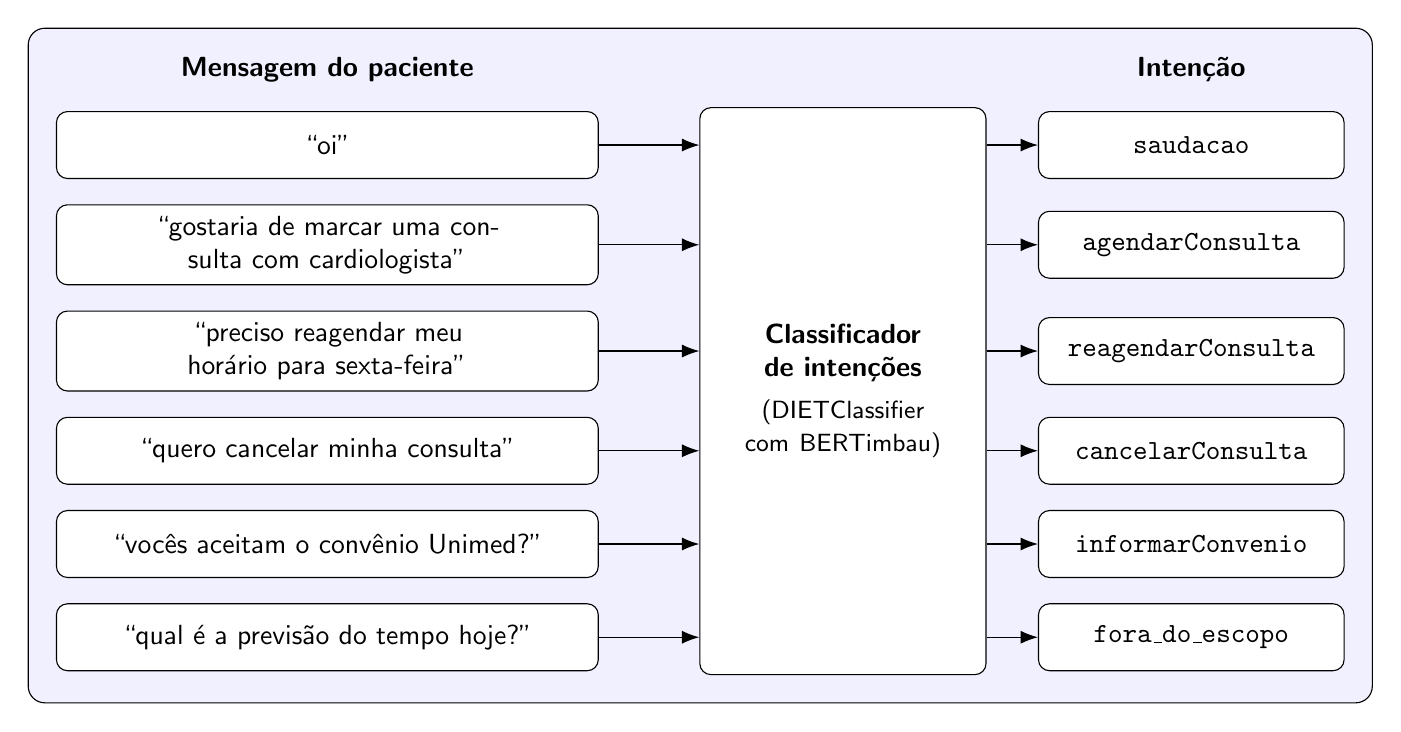
\begin{tikzpicture}[node distance=0.32cm]
\node[msg] (m1) {``oi''};
\node[msg, below=of m1] (m2) {``gostaria de marcar uma consulta com cardiologista''};
\node[msg, below=of m2] (m3) {``preciso reagendar meu horário para sexta-feira''};
\node[msg, below=of m3] (m4) {``quero cancelar minha consulta''};
\node[msg, below=of m4] (m5) {``vocês aceitam o convênio Unimed?''};
\node[msg, below=of m5] (m6) {``qual é a previsão do tempo hoje?''};

\node[rectangle, rounded corners=4pt, draw, fill=white, align=center, font=\bfseries,
      text width=3.4cm, minimum height=7.2cm]
  (clf) at ($(m1.east)!0.5!(m6.east)+(3.1,0)$) {Classificador\\de intenções\\[4pt]
  \normalfont\small (DIETClassifier\\com BERTimbau)};

\foreach \i/\nome in {1/saudacao, 2/agendarConsulta, 3/reagendarConsulta,
                      4/cancelarConsulta, 5/informarConvenio, 6/fora\_do\_escopo} {
  \node[int] (i\i) at ($(clf.east |- m\i)+(2.6,0)$) {\nome};
  \draw[seta] (m\i.east) -- (clf.west |- m\i);
  \draw[seta] (clf.east |- m\i) -- (i\i.west);
}

\node[titulo, above=0.25cm of m1] {Mensagem do paciente};
\node[titulo, above=0.25cm of i1] {Intenção};

\coordinate (topo) at ($(m1.north)+(0,0.7)$);
\begin{scope}[on background layer]
  \node[draw, rounded corners=6pt, fill=blue!6, inner sep=10pt,
        fit=(m1) (m6) (clf) (i1) (i6) (topo)] {};
\end{scope}
\end{tikzpicture}
\end{document}
